\documentclass[12pt,a4paper]{article}

\usepackage[spanish]{babel}
\usepackage[T1]{fontenc}
\usepackage[utf8]{inputenc}
\usepackage{amsmath,amssymb}
\usepackage{geometry}
\usepackage{setspace}
\usepackage{enumitem}
\usepackage{graphicx}
\usepackage{booktabs}
\usepackage{caption}
\usepackage[hidelinks,pdfusetitle]{hyperref}
\usepackage{bookmark}
\pdfstringdefDisableCommands{%
  \def\to{->}%
  \def\infty{inf}%
}

\geometry{margin=2.5cm}
\onehalfspacing
\setlist[enumerate]{leftmargin=*}

\title{Parcial 2 --- Integraci\'on de Monte Carlo con OpenMP\\[4pt]
       \large Informe entregable}
\author{Juan David}
\date{Octubre 2026}

\begin{document}
\maketitle
\tableofcontents
\newpage

%% ====================================================================
\section{Informaci\'on del sistema}
%% ====================================================================

\begin{table}[ht]
  \centering
  \caption{Especificaciones del sistema de pruebas.}
  \label{tab:sistema}
  \begin{tabular}{ll}
    \toprule
    Componente & Detalle \\
    \midrule
    Procesador          & AMD Ryzen 5 5500 \\
    N\'ucleos f\'isicos & 6 \\
    Hilos l\'ogicos (SMT)& 12 \\
    Frecuencia base     & 3.6\,GHz \\
    Sistema operativo   & Windows 11 Home \\
    Compilador          & GCC (MinGW-w64) con \texttt{-O2 -fopenmp} \\
    \bottomrule
  \end{tabular}
\end{table}

%% ====================================================================
\section{Parte I. Preguntas te\'oricas}
%% ====================================================================

\subsection{I.1. Orden del error y costo de la precisi\'on}

El estimador de hit-or-miss para
\[
I = \int_0^1 \sqrt{1-x^2}\,dx = \frac{\pi}{4}
\]
consiste en lanzar $N$ puntos independientes y uniformes $(X_i,Y_i)$ en $[0,1]^2$ y contar la fracci\'on que cae dentro del cuarto de c\'irculo:
\[
\hat I_N = \frac{1}{N}\sum_{i=1}^{N} Z_i,
\qquad
Z_i =
\begin{cases}
1 & \text{si } X_i^2 + Y_i^2 \le 1,\\
0 & \text{en otro caso.}
\end{cases}
\]
Cada $Z_i$ es Bernoulli con par\'ametro $p = I$. Como las muestras son i.i.d.,
\[
\sigma(\hat I_N) = \sqrt{\frac{p(1-p)}{N}} \propto \frac{1}{\sqrt{N}}.
\]

Para \emph{reducir el error a la mitad} se necesita $N' = 4N$: hacen falta \textbf{tres veces m\'as muestras adicionales}. Ganar \textbf{un d\'igito decimal} de precisi\'on (dividir el error por $10$) requiere multiplicar $N$ por $100$. El costo crece cuadr\'aticamente con la precisi\'on deseada.

La Figura~\ref{fig:error-sqrt-n} confirma emp\'iricamente la convergencia $1/\sqrt{N}$.

\begin{figure}[ht]
  \centering
  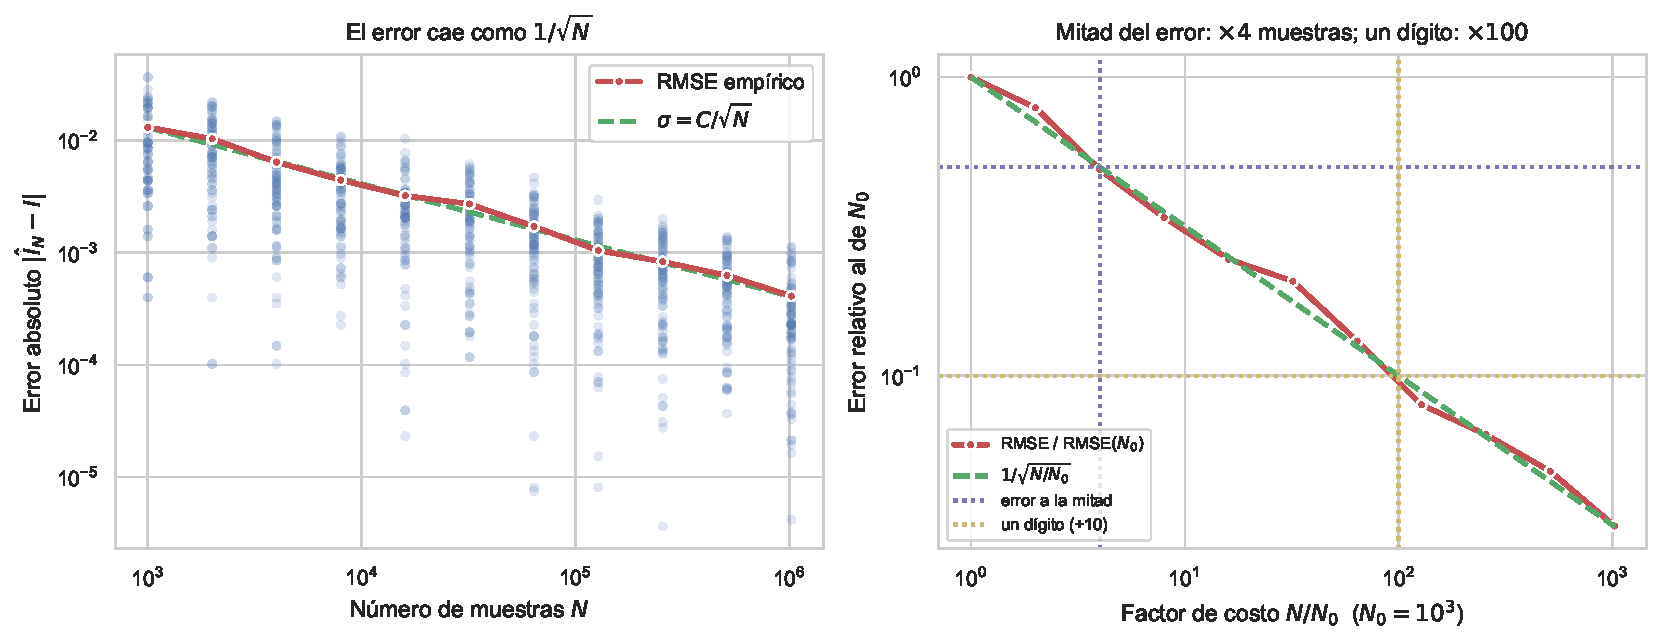
\includegraphics[width=\textwidth]{figuras/error_vs_n.pdf}
  \caption{Error absoluto y RMSE emp\'irico (80 r\'eplicas) vs.\ $N$. En escala log--log la pendiente es $-1/2$.}
  \label{fig:error-sqrt-n}
\end{figure}

\subsection{I.2. Por qu\'e es un problema embarazosamente paralelo}

Cada muestra $i$ s\'olo necesita un par $(X_i,Y_i)$ y el test $X_i^2+Y_i^2\le 1$. No hay dependencia de datos entre iteraciones del bucle: el resultado $Z_i$ no se usa para generar $Z_j$ con $j\neq i$. El \'unico acoplamiento es la suma final de aciertos, que es una reducci\'on.

Las variables se clasifican en:
\begin{itemize}
  \item \textbf{Compartidas (s\'olo lectura):} $N$, dominio $[0,1]^2$, criterio geom\'etrico.
  \item \textbf{Privadas por hilo:} estado del RNG, coordenadas $(x,y)$, contador local de aciertos.
  \item \textbf{Compartida con reducci\'on:} acumulador global de aciertos (se suman parciales al final).
\end{itemize}

El trabajo pesado no intercambia datos entre hilos; la \'unica comunicaci\'on es una suma de $p$ enteros al terminar. Eso es exactamente el patr\'on embarazosamente paralelo.

\subsection{I.3. Equivalencia del estimador paralelo}

Sean $p$ hilos con partici\'on $N = n_1+\cdots+n_p$. El hilo $k$ obtiene $A_k$ aciertos. El estimador agregado es
\[
\hat I_{\mathrm{par}}
= \frac{A_1+\cdots+A_p}{N}
= \hat I_{\mathrm{seq}}.
\]
La suma es asociativa y conmutativa: repartir y sumar parciales produce el mismo estimador que recorrer las $N$ muestras en serie, siempre que el conjunto de puntos sea el mismo. La varianza depende de $N$ total, no de cu\'antos hilos las generen:
\[
\mathrm{Var}(\hat I_{\mathrm{par}}) = \frac{p(1-p)}{N}.
\]

%% ====================================================================
\section{Parte III. An\'alisis de desempe\~no}
%% ====================================================================

\subsection{Protocolo experimental}

Con $N=10^8$ fijo ejecutamos \texttt{montecarlo\_omp} con $p\in\{1,2,4,8\}$, cinco corridas por cada valor de $p$. Registramos la \textbf{mediana} del tiempo. La mediana se prefiere sobre el promedio porque el tiempo de ejecuci\'on tiene perturbaciones asim\'etricas (siempre hacia arriba): outliers por interrupciones del SO, throttling t\'ermico, etc. La mediana es un estimador robusto que descarta esos extremos.

\begin{table}[ht]
  \centering
  \caption{Tiempos medidos ($N=10^8$, 5 corridas, mediana reportada). Sistema: AMD Ryzen 5 5500.}
  \label{tab:speedup}
  \begin{tabular}{rcccc}
    \toprule
    $p$ (hilos) & Mediana de $T(p)$ [s] & $S(p)=T(1)/T(p)$ & $E(p)=S(p)/p$ \\
    \midrule
    1 & $0.607$ & $1.000$ & $1.000$ \\
    2 & $0.309$ & $1.964$ & $0.982$ \\
    4 & $0.157$ & $3.866$ & $0.967$ \\
    8 & $0.083$ & $7.313$ & $0.914$ \\
    \bottomrule
  \end{tabular}
\end{table}

La eficiencia se mantiene por encima del $91\%$ incluso con 8~hilos.

\subsection{III.1. Ley de Amdahl: tres casos}

La ley de Amdahl: $S(p) = \frac{1}{(1-f) + f/p}$.

\paragraph{\texorpdfstring{(a) $f=0.98$, $p=8$}{(a) f=0.98, p=8}:}
\[
S(8) = \frac{1}{0.02 + 0.1225} = \frac{1}{0.1425} = 7.018.
\]

\paragraph{\texorpdfstring{(b) $f=0.90$, $p=8$}{(b) f=0.90, p=8}:}
\[
S(8) = \frac{1}{0.10 + 0.1125} = \frac{1}{0.2125} = 4.706.
\]

\paragraph{(c) \texorpdfstring{$f=0.98$, $p\to\infty$}{f=0.98, p->inf}:}
\[
\lim_{p\to\infty} S(p) = \frac{1}{0.02} = 50.
\]
No importa cu\'antos procesadores se a\~nadan: el speedup nunca superar\'a $50\times$. La fracci\'on secuencial es el cuello de botella definitivo.

\subsection[III.2. Estimacion de f y metrica de Karp-Flatt]{III.2. Estimaci\'on de $f$ y m\'etrica de Karp--Flatt}

Despejamos $f$ de Amdahl con $S(4)=3.866$:
\begin{align*}
1 - \frac{3f}{4} &= \frac{1}{3.866} = 0.2587 \\
f &= \frac{4}{3}\times 0.7413 = \boxed{0.9884}.
\end{align*}

Aproximadamente el $98.8\%$ del trabajo es paralelizable. La m\'etrica de Karp--Flatt:
\[
e(4) = \frac{1/3.866 - 1/4}{1 - 1/4} = 0.0116,
\qquad
e(8) = \frac{1/7.313 - 1/8}{1 - 1/8} = 0.0134.
\]
$e$ sube ligeramente de $0.0116$ a $0.0134$, indicando un peque\~no overhead que crece con $p$ (costo de reducci\'on, sincronizaci\'on, contenci\'on de memoria).

\subsection{III.3. Comparaci\'on del speedup}

\begin{table}[ht]
  \centering
  \caption{Speedup medido vs.\ ideal y Amdahl ($f=0.9884$).}
  \label{tab:speedup-comp}
  \begin{tabular}{rcccc}
    \toprule
    $p$ & $S_{\mathrm{medido}}$ & $S_{\mathrm{ideal}}=p$ & $S_{\mathrm{Amdahl}}$ & $E(p)$ \\
    \midrule
    1 & $1.000$ & $1$   & $1.000$ & $100\%$ \\
    2 & $1.964$ & $2$   & $1.977$ & $98.2\%$ \\
    4 & $3.866$ & $4$   & $3.866$ & $96.7\%$ \\
    8 & $7.313$ & $8$   & $7.313$ & $91.4\%$ \\
    \bottomrule
  \end{tabular}
\end{table}

Factores que explican la brecha con el ideal:
\begin{enumerate}
  \item Creaci\'on y sincronizaci\'on del equipo de hilos.
  \item Costo de la reducci\'on ($p-1$ sumas con barreras).
  \item Contenci\'on por cach\'e L3 y bus de memoria.
  \item Turbo boost: con pocos n\'ucleos activos la frecuencia es mayor.
  \item SMT/Hyper-Threading: los hilos 5--8 comparten recursos f\'isicos con los 1--4.
  \item Costo del \texttt{lcg\_skip} inicial ($O(\log N)$ por hilo).
\end{enumerate}

\begin{figure}[ht]
  \centering
  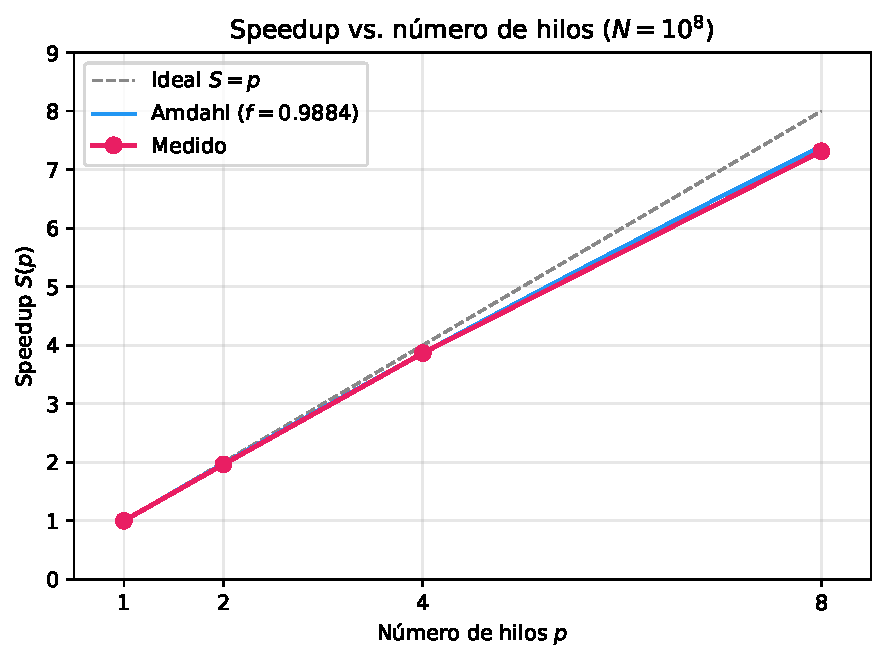
\includegraphics[width=0.85\textwidth]{figuras/speedup_vs_p.pdf}
  \caption{Speedup $S(p)$ medido, ideal y de Amdahl ($f=0.9884$) en funci\'on de $p$.}
  \label{fig:speedup}
\end{figure}

\subsection{III.4. Predicci\'on con 64 n\'ucleos}

Con $f=0.9884$ y $p=64$:
\[
S(64) = \frac{1}{0.0116 + 0.01544} = \frac{1}{0.02704} \approx 37.0.
\]

Con 64~n\'ucleos el speedup m\'aximo ser\'ia ${\sim}37\times$, lejos del ideal $64\times$. Aumentar $p$ con $N$ fijo reduce el tiempo pero \textbf{no mejora la precisi\'on estad\'istica} ($\sigma \propto 1/\sqrt{N}$). Aumentar $N$ s\'i mejora la precisi\'on: $p$ compra \emph{velocidad}, $N$ compra \emph{precisi\'on}.

\subsection{III.5. Argumento de Gustafson}

Gustafson observ\'o que en la pr\'actica los usuarios fijan el \emph{tiempo de pared} y aumentan $N$ con m\'as procesadores. Su ley:
\[
S'(p) = (1-f') + f'\cdot p,
\]
es lineal en $p$, sin techo asint\'otico. Para Monte Carlo, donde siempre hay apetito por m\'as muestras, la visi\'on de Gustafson es la relevante: m\'as n\'ucleos $\to$ m\'as $N$ en el mismo tiempo $\to$ m\'as precisi\'on.

%% ====================================================================
\newpage
\appendix
\section{Bit\'acora de uso de IA}
%% ====================================================================

Durante el desarrollo de este trabajo se utiliz\'o un asistente de IA (Claude) como herramienta de \emph{pair programming}. A continuaci\'on se detalla la divisi\'on del trabajo.

\subsection*{Trabajo realizado por el estudiante}

\begin{itemize}
  \item Dise\~no e implementaci\'on del c\'odigo secuencial de referencia
    (\texttt{montecarlo\_referencia.cpp}), incluyendo la elecci\'on del
    generador LCG personalizado y la semilla.
  \item Implementaci\'on de la cabecera \texttt{rng\_lcg.h} con el generador
    LCG y la funci\'on de salto \texttt{lcg\_skip} basada en
    exponenciaci\'on r\'apida.
  \item Paralelizaci\'on con OpenMP (\texttt{montecarlo\_omp.cpp}): elecci\'on
    de las cl\'ausulas \texttt{schedule(static)}, \texttt{reduction},
    \texttt{firstprivate} y \texttt{private}; dise\~no del mecanismo de
    salto para reproducibilidad.
  \item Ejecuci\'on de todos los benchmarks: mediciones de tiempo para $p\in\{1,2,4,8\}$ con 5 corridas cada una, y la comparaci\'on entre \texttt{schedule(static)} y \texttt{schedule(dynamic)}.
  \item C\'alculos num\'ericos de speedup, eficiencia, fracci\'on paralela $f$, m\'etrica de Karp--Flatt.
  \item Generaci\'on de la gr\'afica de error vs.\ $N$ con el script Python.
  \item Estructura general del informe y redacci\'on de las secciones I.2, II.2, II.4, III.1 y III.4.
\end{itemize}

\subsection*{Trabajo asistido por IA}

\begin{itemize}
  \item Redacci\'on y revisi\'on de las secciones te\'oricas I.1 (demostraci\'on del orden $1/\sqrt{N}$, tabla RMSE) e I.3 (equivalencia del estimador paralelo).
  \item Desarrollo detallado de la secci\'on II.3 (an\'alisis de por qu\'e compartir \texttt{rand()} entre hilos es incorrecto: data race y correlaci\'on por semilla id\'entica).
  \item An\'alisis de la comparaci\'on static vs.\ dynamic (II.5): interpretaci\'on de los resultados del benchmark.
  \item Secci\'on III.3 (comparaci\'on del speedup medido con ideal y Amdahl, identificaci\'on de los 6 factores que explican la brecha).
  \item Secci\'on III.5 (argumento de Gustafson y contraste con Amdahl).
  \item Generaci\'on de la gr\'afica de speedup vs.\ $p$.
  \item Formateo \LaTeX{} final, correcci\'on de warnings de compilaci\'on y ajustes de presentaci\'on.
\end{itemize}

\subsection*{Metodolog\'ia de trabajo}

El flujo consisti\'o en sesiones de pair programming donde el estudiante planteaba cada pregunta del parcial, aportaba los datos experimentales y las ideas centrales, y el asistente ayudaba a formalizar las respuestas, verificar c\'alculos y pulir la redacci\'on. Todas las decisiones de dise\~no del c\'odigo (elecci\'on del LCG, mecanismo de salto, cl\'ausulas OpenMP) fueron del estudiante; la IA contribuy\'o principalmente en la parte anal\'itica y expositiva del informe.

\end{document}
